\subsubsection{LINPACK}
\\
The energy, delay and area estimates for each architecture / frequency combination is given in TABLE IV.
In Fig. 4, Fig. 5 we show the Power-Delay and Area-Delay plot for Linpack.

\begin{table}[h!]
\caption{Energy / Delay / Area for each architecture/frequency combination}
\begin{center}
{\begin{tabular}{c | c   c   c   c    c   c}
\hline
LINPACK &1x2 &1x0 &2x0 &2x2 &4x2 &4x0 \\ [1ex]
\hline
Frequency (MHz) & 45.45& 41.67& 41.67& 41.67&41.67 & 38.4\\[1ex]
Energy (mJ) &18.92 &11.47 &22.75 &10.28 &29.53 &11.07 \\ [1ex]

Delay (ms)& 56.48& 43.65& 55.63& 37.68& 51.64& 38.71\\[1ex] 
Area (mm^2)& 27.5& 25.5& 30.8& 27& 36.2& 28.9\\[1ex]
\hline

\end{tabular}}
\label{diffstruc}
\end{center}
\end{table}


\begin{figure}[h!]
{\centering \resizebox*{6in}{4in}{\includegraphics{lpp.ps}} \par}
\caption{Power-Delay plot for LINPACK}
\end{figure}

\begin{figure}[h!]
{\centering \resizebox*{6in}{4in}{\includegraphics{lpa.ps}} \par}
\caption{Area-Delay plot for LINPACK}
\end{figure}


